\documentclass[UTF8,a4paper,12pt,fontset=none]{ctexart}

\usepackage{geometry}
\usepackage{graphicx}
\usepackage{booktabs}
\usepackage{array}
\usepackage{float}
\usepackage{hyperref}
\usepackage{amsmath}
\usepackage{amssymb}
\usepackage{enumitem}
\usepackage{xcolor}
\usepackage{caption}
\usepackage{subcaption}
\usepackage{fancyhdr}

\geometry{left=2.6cm,right=2.6cm,top=2.6cm,bottom=2.6cm}
\setlength{\parskip}{0.55em}
\setlength{\parindent}{2em}
\setlength{\headheight}{15pt}
\definecolor{ThemeBlue}{HTML}{1F4E79}
\definecolor{LightBlue}{HTML}{EAF2F8}
\definecolor{SoftGray}{HTML}{F6F8FA}
\definecolor{DeepGray}{HTML}{3C4856}
\hypersetup{colorlinks=true,linkcolor=ThemeBlue,urlcolor=ThemeBlue,citecolor=ThemeBlue}
\setCJKmainfont{Songti SC}
\setCJKsansfont{Heiti SC}
\setCJKmonofont{Hiragino Sans GB}
\captionsetup{font=small,labelfont=bf}
\renewcommand{\arraystretch}{1.18}
\setlist{leftmargin=2em}
\emergencystretch=3em

\pagestyle{fancy}
\fancyhf{}
\lhead{大数据处理课程期末项目}
\rhead{短视频主题偏好分析与推荐策略优化}
\cfoot{\thepage}

\newcommand{\reporttitle}{基于 Tsinghua ShortVideo Dataset 的短视频主题偏好分析与推荐策略优化研究}

\begin{document}

\begin{titlepage}
\thispagestyle{empty}
\centering
\vspace*{1.7cm}
{\Large \textcolor{ThemeBlue}{大数据处理课程期末项目}\par}
\vspace{1.2cm}
{\Huge \bfseries 短视频主题偏好分析与推荐策略优化研究\par}
\vspace{0.35cm}
{\Large \bfseries 基于 Tsinghua ShortVideo Dataset 的实证分析\par}
\vspace{1.2cm}
\textcolor{ThemeBlue}{\rule{0.78\textwidth}{1.2pt}}
\vspace{1.5cm}

\begin{minipage}{0.84\textwidth}
\large
\begin{tabular}{>{\bfseries}p{3.1cm}p{9.3cm}}
课程名称 & 大数据处理 \\
学院 & 国家网络空间安全学院 \\
指导教师 & 汪润 \\
小组成员 & 梁珂、方家烨、李俊婕、刘翔 \\
项目主题 & 短视频主题偏好分析、关联规则挖掘与推荐策略优化 \\
\end{tabular}
\end{minipage}

\vfill
{\large \today\par}
\end{titlepage}

\begin{abstract}
短视频推荐系统面对的是高频曝光、弱反馈密集、内容主题多样的行为数据。课程项目围绕“如何从用户观看和互动行为中识别主题偏好，并将可解释的群体规律用于推荐排序”展开，基于 Tsinghua ShortVideo Dataset 的抽样交互数据，构建了从数据清洗、主题行为统计、用户主题画像、关联规则挖掘到推荐策略评估的完整流程。实验将原始多标签曝光记录聚合为用户-视频级交互，构造观看比例、有效观看、互动反馈和负反馈等特征，并按用户时间顺序划分训练集与测试集，避免偏好构建和规则挖掘阶段使用测试行为。推荐实验设置了两个可比较方案：baseline 只使用用户历史主题偏好和视频热门度，rule-enhanced 在此基础上引入分群主题成功率、关联规则质量、相似主题迁移、标签匹配和负反馈风险。实验结果显示，rule-enhanced 在 HitRate@10、Precision@10、Recall@10 和 ThemeMatch@10 上均超过 baseline，说明主题级规则和群体反馈可以为个体历史偏好提供有效补充。项目同时给出 Python 本地流水线、Spark 主题统计与 FP-Growth 实现、Hive 离线数仓 SQL，以及可复现的结果表和可视化图表。
\end{abstract}

\noindent\textbf{关键词：} 短视频推荐；主题偏好；用户画像；关联规则；推荐评估；Spark；Hive

\vspace{0.8em}
\noindent\colorbox{LightBlue}{\parbox{0.96\textwidth}{
\textbf{核心结果。}
清洗后数据包含 129,483 条交互、6,654 名用户、31,496 个视频和 36 个一级主题。训练集挖掘出 7,658 条主题/标签/用户属性到行为的关联规则。与 baseline 相比，rule-enhanced 的 HitRate@10 从 0.023013 提升至 0.026107，Recall@10 从 0.008712 提升至 0.009914，ThemeMatch@10 从 0.412038 提升至 0.423806。
}}

\newpage
\tableofcontents
\newpage

\section{研究背景与问题定义}

短视频平台的内容分发高度依赖推荐系统。与传统长视频或新闻推荐相比，短视频交互具有曝光频率高、单次观看时间短、反馈信号稀疏但类型丰富的特点。用户可能没有显式评分，却会通过观看时长、是否完整观看、点赞、收藏、评论、转发和负反馈等行为留下偏好线索。对于课程项目而言，这类数据适合用来训练完整的大数据处理能力：需要从原始行为表中清洗字段、构建中间表、聚合主题统计、挖掘行为规则，并将结果放回推荐排序中验证效果。

本文关注的核心问题不是“哪一个视频最热门”，而是“不同主题如何影响用户行为，以及这些主题规律能否转化为推荐增益”。为回答这一问题，项目将视频一级主题作为主要分析对象，把用户属性、视频标签和行为反馈纳入同一个统计框架。主题行为统计用于观察不同内容类型的观看深度和互动差异，用户主题偏好画像用于描述个体兴趣，关联规则用于刻画标签、主题、用户分组和行为之间的可解释关系，推荐实验则检验这些规律是否能改善 Top-10 离线推荐结果。

课程报告的贡献体现在三个层面。数据层面，项目完成了从原始抽样表到用户-视频级交互表的清洗和去重，处理了布尔字段、观看比例、年龄分组、价格分组和主题映射等问题。方法层面，项目设计了可解释的偏好得分和 rule-enhanced 重排序方案，将主题偏好、热门度、分群反馈、规则质量、标签匹配和负反馈风险统一到推荐分数中。工程层面，项目同时保留本地 Python 流水线、Spark 实现和 Hive SQL，使报告结论可以追溯到代码和输出文件。

\section{数据来源与实验边界}

\subsection{数据来源}

实验使用 Tsinghua ShortVideo Dataset 的小规模抽样数据。完整数据集包含大规模视频文件、多模态特征和行为记录，体量不适合在普通本地环境完整下载和上传。因此，本项目将原始抽样数据保留在本地 \path{data_raw/shortvideo_tiny/}，在仓库中只提交清洗后的轻量表、统计结果、推荐结果、图表、脚本和报告。推荐实验主要使用 \path{interaction_sampled.csv} 与 \path{categories_cn_en.csv}，前者提供用户曝光、观看、互动、视频属性和用户属性，后者提供类别 ID 与中英文主题名称的映射。

这种数据取舍符合课程项目的目标。完整视频文件更适合多模态内容理解任务，而本文的重点是大数据处理流程和基于主题行为的推荐策略验证。抽样数据能够支持清洗、聚合、规则挖掘、推荐评估和可视化展示，也能保证实验在本地机器上可重复运行。

\subsection{字段结构}

交互表同时包含用户、视频、时间、行为和内容标签等字段。表~\ref{tab:fields} 汇总了本文使用的核心字段。

\begin{table}[H]
\centering
\caption{实验使用的核心字段}
\label{tab:fields}
\begin{tabular}{p{2.5cm}p{3.8cm}p{7.6cm}}
\toprule
字段类别 & 字段名 & 用途 \\
\midrule
用户标识 & \texttt{user\_id} & 构建用户画像，按用户划分训练集和测试集 \\
视频标识 & \texttt{pid} & 作为推荐候选和命中评估对象 \\
时间字段 & \texttt{exposed\_time} & 保留用户行为顺序，避免随机切分造成泄露 \\
观看行为 & \texttt{watch\_time}, \texttt{duration} & 计算观看比例和有效观看 \\
互动行为 & \texttt{cvm\_like}, \texttt{comment}, \texttt{collect}, \texttt{forward} & 表示点赞、评论、收藏和转发等正向反馈 \\
负反馈 & \texttt{hate} & 推荐排序中的风险惩罚信号 \\
主题与标签 & \texttt{root\_id}, \texttt{category\_id}, \texttt{tag\_name} & 构建主题统计、规则事务和标签匹配特征 \\
用户属性 & \texttt{gender}, \texttt{age}, \texttt{fre\_city\_level} & 支持性别、年龄段和城市等级分组分析 \\
\bottomrule
\end{tabular}
\end{table}

\subsection{实验边界}

抽样实验不能直接等同于工业推荐系统评测。样本只覆盖一段有限时间窗口，候选视频也来自训练集中出现过的视频，因此本文不评价新视频冷启动和长期兴趣漂移。离线指标的绝对值会受到样本规模、测试集正反馈稀疏性和候选集合限制影响。报告更关注同一数据切分下两个推荐方案的相对差异，即 rule-enhanced 是否能稳定超过只使用个体偏好和热门度的 baseline。

实验还设置了防泄露边界。用户主题偏好、关联规则、候选视频集合、视频热门度和用户分群统计全部由训练集构建，测试集只用于评估。该设计使推荐方案不能提前看到用户后续行为，评估结果更接近真实推荐系统中的时间顺序场景。

\section{数据清洗与特征构建}

\subsection{用户-视频级交互表}

原始数据中同一次曝光可能因多个标签而对应多行记录，如果直接统计会重复计算曝光和互动。项目以 \texttt{user\_id}、\texttt{pid} 和 \texttt{exposed\_time} 为联合键聚合到用户-视频级粒度。聚合时，观看时长、视频时长、用户属性和主题字段保留首个非空值，点赞、收藏、评论、转发、负反馈和有效观看取逻辑或，标签字段按出现顺序合并为以竖线分隔的标签串。该处理保留了标签信息，又避免了多标签重复行放大主题曝光量。

行为字段被统一转为布尔值，观看时长和视频时长转为数值。有效观看由 \(watch\_time>3\) 派生，观看比例按式~\ref{eq:watch-ratio} 计算，并截断到 \([0,1]\) 区间。视频时长缺失或小于等于 0 时，观看比例置为 0。年龄被划分为 \texttt{<=18}、\texttt{19-25}、\texttt{26-35}、\texttt{36-45}、\texttt{46-60} 和 \texttt{60+}，缺失值进入 \texttt{unknown} 分组。

\begin{equation}
\label{eq:watch-ratio}
WatchRatio=\min\left(\max\left(\frac{watch\_time}{duration},0\right),1\right)
\end{equation}

\subsection{交互偏好得分}

用户对视频主题的偏好不能只依赖是否点击或是否点赞。短视频场景下，观看比例能够反映用户是否停留，点赞、收藏、评论和转发代表更强的正向反馈，负反馈则表示排斥。项目将这些信号合成为交互得分 \(S\)，用于后续用户-主题画像：

\begin{equation}
\label{eq:interaction-score}
S = 0.45R + 0.20E + 0.15L + 0.10C + 0.05M + 0.08F - 0.20H
\end{equation}

式中，\(R\) 表示观看比例，\(E\) 表示有效观看，\(L\) 表示点赞，\(C\) 表示收藏，\(M\) 表示评论，\(F\) 表示转发，\(H\) 表示负反馈。对同一用户在同一主题下的交互得分求和，即可得到用户-主题偏好强度。这个分数不是工业推荐模型中的学习参数，而是课程项目中可解释、可复现的偏好刻画方式。

\subsection{训练测试切分}

项目按用户内部时间顺序进行训练测试切分。对交互数不少于 3 条的用户，前 80\% 行为进入训练集，后 20\% 行为进入测试集；交互过少的用户只进入训练集，不参与测试评估。最终数据规模见表~\ref{tab:scale}。

\begin{table}[H]
\centering
\caption{清洗后数据规模}
\label{tab:scale}
\small
\begin{tabular}{lrrrrrrr}
\toprule
口径 & 清洗交互 & 训练交互 & 测试交互 & 用户 & 视频 & 主题 & 规则 \\
\midrule
数量 & 129,483 & 101,690 & 27,793 & 6,654 & 31,496 & 36 & 7,658 \\
\bottomrule
\end{tabular}
\end{table}

\section{方法设计}

\subsection{整体流程}

项目的处理流程从原始抽样数据开始，经过字段清洗、用户-视频级聚合、训练测试切分、主题统计、用户画像、规则挖掘、推荐排序和离线评估，最终输出结果表与图表。图~\ref{fig:pipeline} 展示了主要阶段以及训练集与测试集的使用边界。

\begin{figure}[H]
\centering
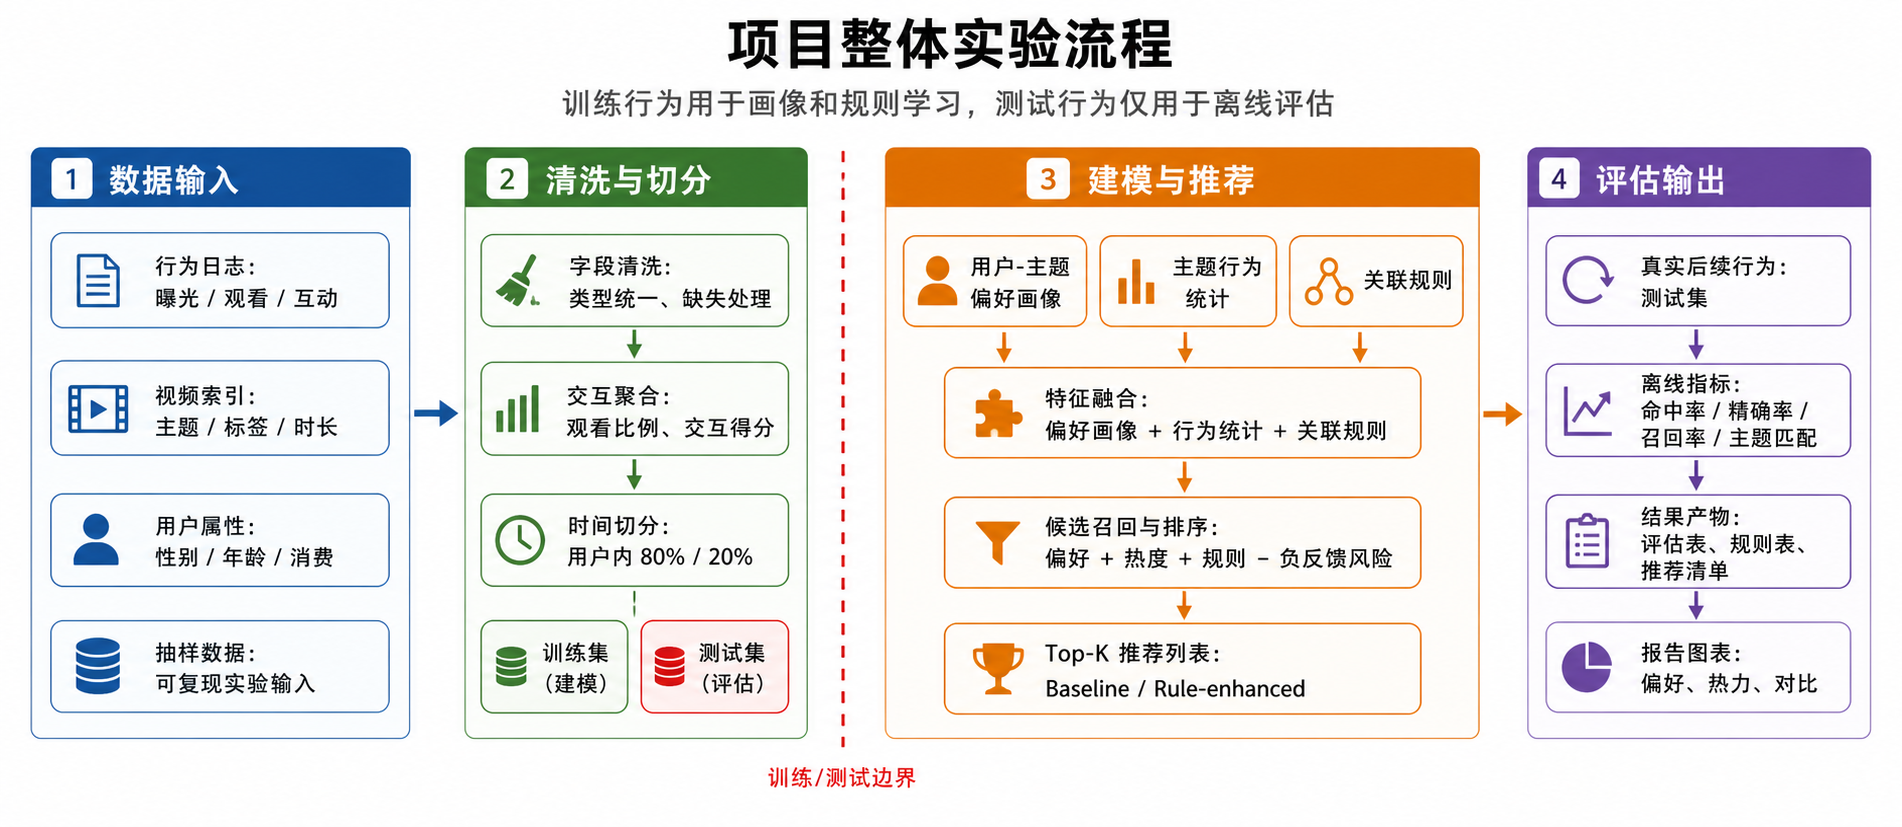
\includegraphics[width=0.98\textwidth]{../../output/figures/method_pipeline_overview.png}
\caption{项目整体实验流程}
\label{fig:pipeline}
\end{figure}

\subsection{主题行为统计}

主题行为统计按一级主题聚合训练集记录，计算曝光数、用户数、视频数、平均观看时长、平均观看比例、有效观看率、点赞率、收藏率、评论率、转发率和负反馈率。这部分结果用于回答不同主题是否存在观看深度和互动差异，也为后续规则挖掘和推荐解释提供背景。

\subsection{关联规则挖掘}

关联规则将每条用户-视频交互转化为一个事务。事务项包括主题项、标签项、用户属性项和行为项，例如 \texttt{theme=9}、\texttt{tag=搞笑}、\texttt{age\_group=19-25}、\texttt{behavior=like}。本地 Python 流水线采用轻量 Apriori-style 统计方法，计算一阶或二阶前件到行为后件的支持度、置信度和提升度；Spark 脚本则使用 \texttt{pyspark.ml.fpm.FPGrowth} 给出分布式环境下的规则挖掘版本。

\begin{equation}
Support(A\Rightarrow B)=\frac{count(A\cup B)}{N}
\end{equation}

\begin{equation}
Confidence(A\Rightarrow B)=\frac{count(A\cup B)}{count(A)}
\end{equation}

\begin{equation}
Lift(A\Rightarrow B)=\frac{Confidence(A\Rightarrow B)}{Support(B)}
\end{equation}

关联规则不被解释为因果关系。本文只把它作为推荐中的统计辅助信号：与正向行为相关且支持数、置信度和提升度足够高的规则进入主题质量或标签匹配特征；与负反馈相关的规则进入风险惩罚特征。

\subsection{推荐方案}

Baseline 是对照方法，只使用用户历史主题偏好和视频热门度。候选视频来自训练集中出现过、且用户未看过的视频。对用户 \(u\) 和候选视频 \(i\)，基础分数定义为：

\begin{equation}
Score_{base}(u,i)=0.82P(u,t_i)+0.18Pop(i)
\end{equation}

其中，\(P(u,t_i)\) 是用户对候选视频主题 \(t_i\) 的归一化偏好分，\(Pop(i)\) 是候选视频在训练集中的归一化热门度。Baseline 的优势是简单和可解释，局限是只利用个体历史与整体热度，无法利用用户分群和标签规则。

Rule-enhanced 在 baseline 基础上进行重排序。它保留个体偏好作为主体，同时引入五类训练集信号：用户分群主题成功率 \(G\)、主题规则质量 \(Q\)、相似主题迁移 \(Sim\)、标签规则匹配 \(Tag\) 和负反馈风险 \(Risk\)。最终分数为：

\begin{align}
Score_{enh}(u,i)=&0.58Score_{base}(u,i)+0.16G(u,t_i)+0.11Q(t_i) \\
&+0.08Sim(u,t_i)+0.09Pop(i)+0.05Tag(u,i)-0.07Risk(u,t_i)
\end{align}

分群主题成功率来自性别、年龄段和城市等级下的主题反馈统计，并通过全局主题表现平滑。相似主题迁移由用户高偏好主题共现关系估计。标签规则匹配用于捕捉候选视频标签与用户历史正反馈标签的重合。负反馈风险用于降低用户已明确排斥或规则层面风险较高的主题。

\section{实验结果与分析}

\subsection{主题行为差异}

高曝光主题的统计结果见表~\ref{tab:theme-summary}。影视和短剧是样本中曝光最多的主题，但其平均观看比例低于搞笑、生活、亲子和明星娱乐。亲子主题的平均观看比例达到 0.5629，有效观看率为 0.7448，说明该主题虽然曝光规模低于影视和短剧，但观看完整度更高。音乐和游戏的点赞率相对更高，表明互动反馈和观看深度不一定同步变化。

\begin{table}[H]
\centering
\caption{高曝光主题行为统计}
\label{tab:theme-summary}
\begin{tabular}{lrrrr}
\toprule
主题 & 曝光数 & 平均观看比例 & 有效观看率 & 点赞率 \\
\midrule
影视和短剧 & 18,469 & 0.3704 & 0.7283 & 0.0177 \\
搞笑 & 11,623 & 0.5114 & 0.7607 & 0.0206 \\
美食 & 7,298 & 0.4290 & 0.6905 & 0.0148 \\
生活 & 6,298 & 0.5239 & 0.7191 & 0.0168 \\
亲子 & 4,656 & 0.5629 & 0.7448 & 0.0174 \\
游戏 & 4,653 & 0.4965 & 0.7423 & 0.0258 \\
音乐 & 4,411 & 0.3529 & 0.6629 & 0.0329 \\
明星娱乐 & 3,634 & 0.5167 & 0.7664 & 0.0261 \\
\bottomrule
\end{tabular}
\end{table}

图~\ref{fig:watch-time} 与图~\ref{fig:interaction-rate} 从平均观看时长和互动率两个角度展示主题差异。观看时长较长的主题不一定拥有最高点赞率，这说明推荐排序如果只依赖单一行为信号，容易偏向某类反馈而忽略用户对内容的真实停留情况。

\begin{figure}[H]
\centering
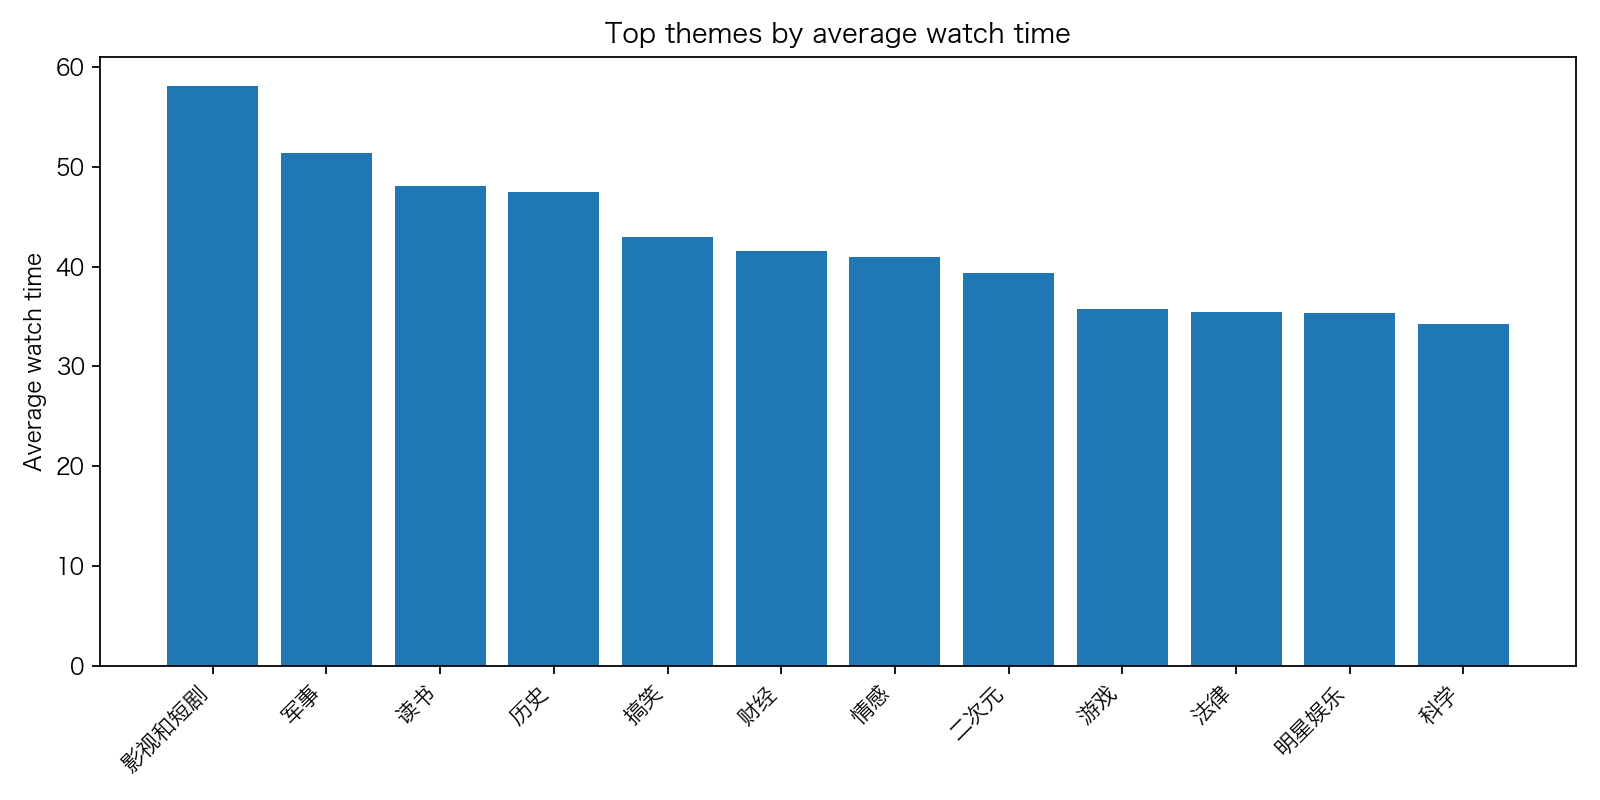
\includegraphics[width=0.86\textwidth]{../../output/figures/top_theme_watch_time.png}
\caption{不同主题平均观看时长对比}
\label{fig:watch-time}
\end{figure}

\begin{figure}[H]
\centering
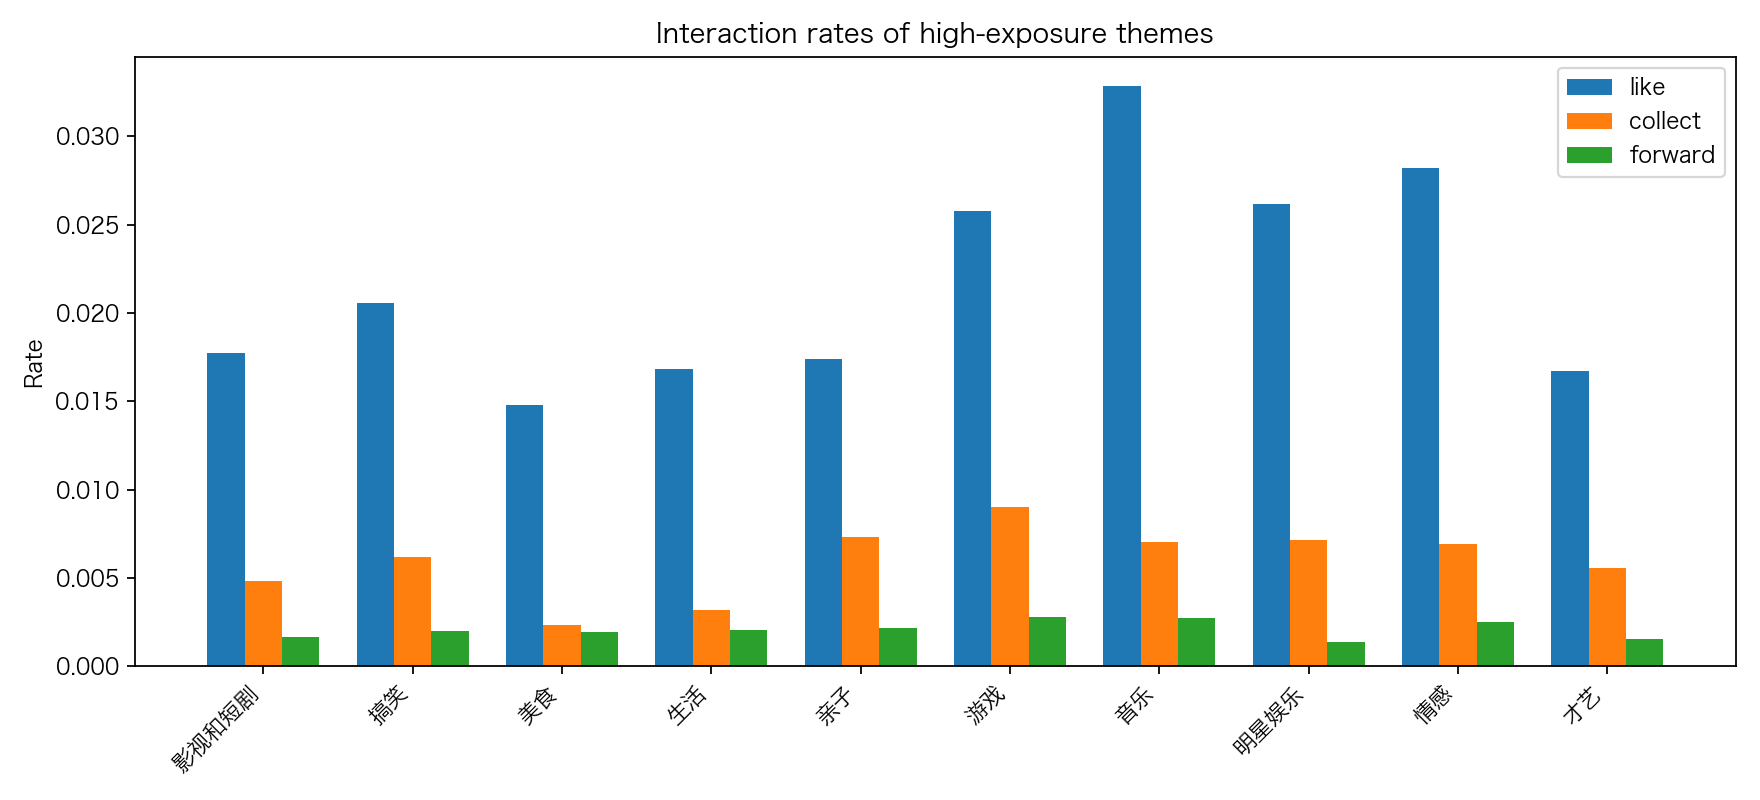
\includegraphics[width=0.86\textwidth]{../../output/figures/theme_interaction_rates.png}
\caption{高曝光主题互动率对比}
\label{fig:interaction-rate}
\end{figure}

\subsection{关联规则结果}

训练集共挖掘出 7,658 条规则。表~\ref{tab:rules} 列出部分高提升度规则。样例显示，部分标签和用户分组组合与点赞行为具有明显高于全局平均的关系。例如，\texttt{tag=一人分饰多角} 到点赞行为的提升度为 5.2541，表示带有该标签的交互中点赞发生概率相对全局点赞概率更高；\texttt{age\_group=19-25} 与若干主题组合也多次出现在高提升度规则中，说明年轻用户在部分主题下存在更强的点赞倾向。

\begin{table}[H]
\centering
\caption{关联规则样例}
\label{tab:rules}
\begin{tabular}{p{6.2cm}p{3.2cm}rrr}
\toprule
前件 & 后件 & 支持数 & 置信度 & 提升度 \\
\midrule
\texttt{tag=一人分饰多角} & \texttt{behavior=like} & 20 & 0.1070 & 5.2541 \\
\texttt{age\_group=19-25 \& theme=20} & \texttt{behavior=like} & 49 & 0.0729 & 3.5821 \\
\texttt{tag=捕娱计划} & \texttt{behavior=like} & 24 & 0.0706 & 3.4677 \\
\texttt{age\_group=19-25 \& theme=19} & \texttt{behavior=like} & 24 & 0.0694 & 3.4076 \\
\texttt{age\_group=19-25 \& city\_level=二线城市} & \texttt{behavior=like} & 203 & 0.0691 & 3.3955 \\
\bottomrule
\end{tabular}
\end{table}

这些规则的价值不在于替代个体偏好，而在于补充个体偏好。对于历史行为较少的用户，分群规则提供了平滑参考；对于主题偏好相近但标签差异较大的候选视频，标签规则可以提供细粒度区分；对于负反馈风险较高的主题，规则能够阻止纯热门视频进入推荐列表。

\subsection{推荐效果}

测试集中满足有效观看、点赞、收藏、评论或转发任一条件且没有负反馈的记录被视为正反馈。评估指标包括 HitRate@10、Precision@10、Recall@10 和 ThemeMatch@10。结果见表~\ref{tab:evaluation}。

\begin{table}[H]
\centering
\caption{推荐效果评估}
\label{tab:evaluation}
\begin{tabular}{lrrrr}
\toprule
方法 & HitRate@10 & Precision@10 & Recall@10 & ThemeMatch@10 \\
\midrule
Baseline & 0.023013 & 0.002398 & 0.008712 & 0.412038 \\
Rule-enhanced & 0.026107 & 0.002649 & 0.009914 & 0.423806 \\
\bottomrule
\end{tabular}
\end{table}

相对提升见表~\ref{tab:relative-improvement}。Rule-enhanced 在四项指标上都获得提升，其中 HitRate@10 提升 13.44\%，Recall@10 提升 13.80\%。ThemeMatch@10 的提升幅度较小，但它反映的是推荐主题与测试正反馈主题的一致程度，能够说明增强策略没有仅靠热门视频获得偶然命中，而是在主题层面更贴近用户后续兴趣。

\begin{table}[H]
\centering
\caption{Rule-enhanced 相对 Baseline 的提升幅度}
\label{tab:relative-improvement}
\begin{tabular}{lrrr}
\toprule
指标 & Baseline & Rule-enhanced & 相对提升 \\
\midrule
HitRate@10 & 0.023013 & 0.026107 & 13.44\% \\
Precision@10 & 0.002398 & 0.002649 & 10.47\% \\
Recall@10 & 0.008712 & 0.009914 & 13.80\% \\
ThemeMatch@10 & 0.412038 & 0.423806 & 2.86\% \\
\bottomrule
\end{tabular}
\end{table}

\begin{figure}[H]
\centering
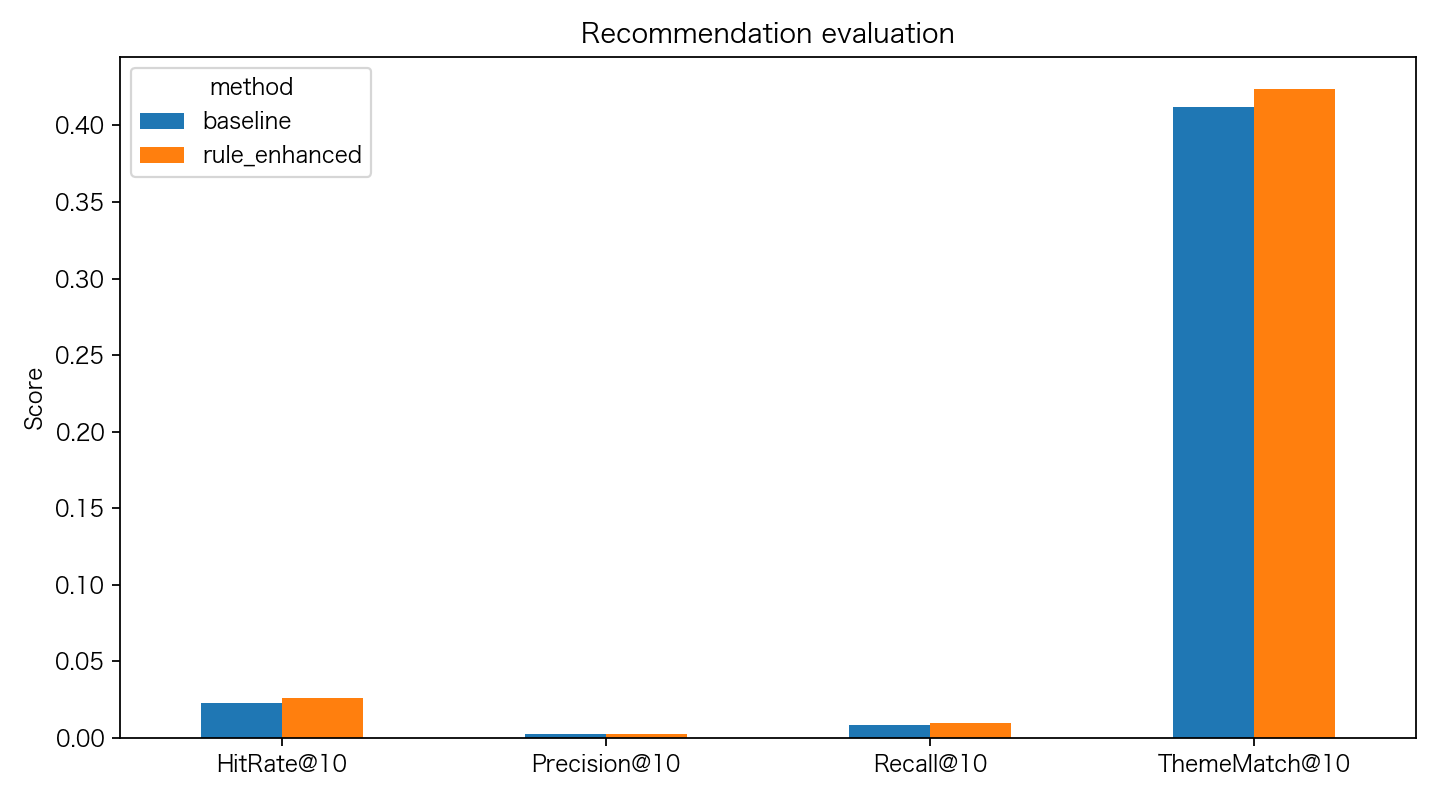
\includegraphics[width=0.82\textwidth]{../../output/figures/recommendation_evaluation.png}
\caption{Baseline 与 Rule-enhanced 推荐效果对比}
\label{fig:evaluation}
\end{figure}

指标绝对值不高，主要原因是抽样数据规模有限，测试集中每个用户的正反馈视频较少，候选集合又受到训练集出现视频的限制。在这种约束下，rule-enhanced 仍能稳定超过 baseline，说明规则增强特征没有破坏个体偏好主体，反而在个体历史不足或主题相近时提供了有效补充。

\subsection{用户分群偏好}

图~\ref{fig:heatmap} 展示了性别与主题之间的偏好差异。不同用户分组对主题的响应并不一致，这为分群主题成功率进入推荐排序提供了数据依据。分群特征不应被理解为对用户兴趣的固定刻板划分，它在本文中只作为训练集统计信号，用于缓解个体历史稀疏问题。

\begin{figure}[H]
\centering
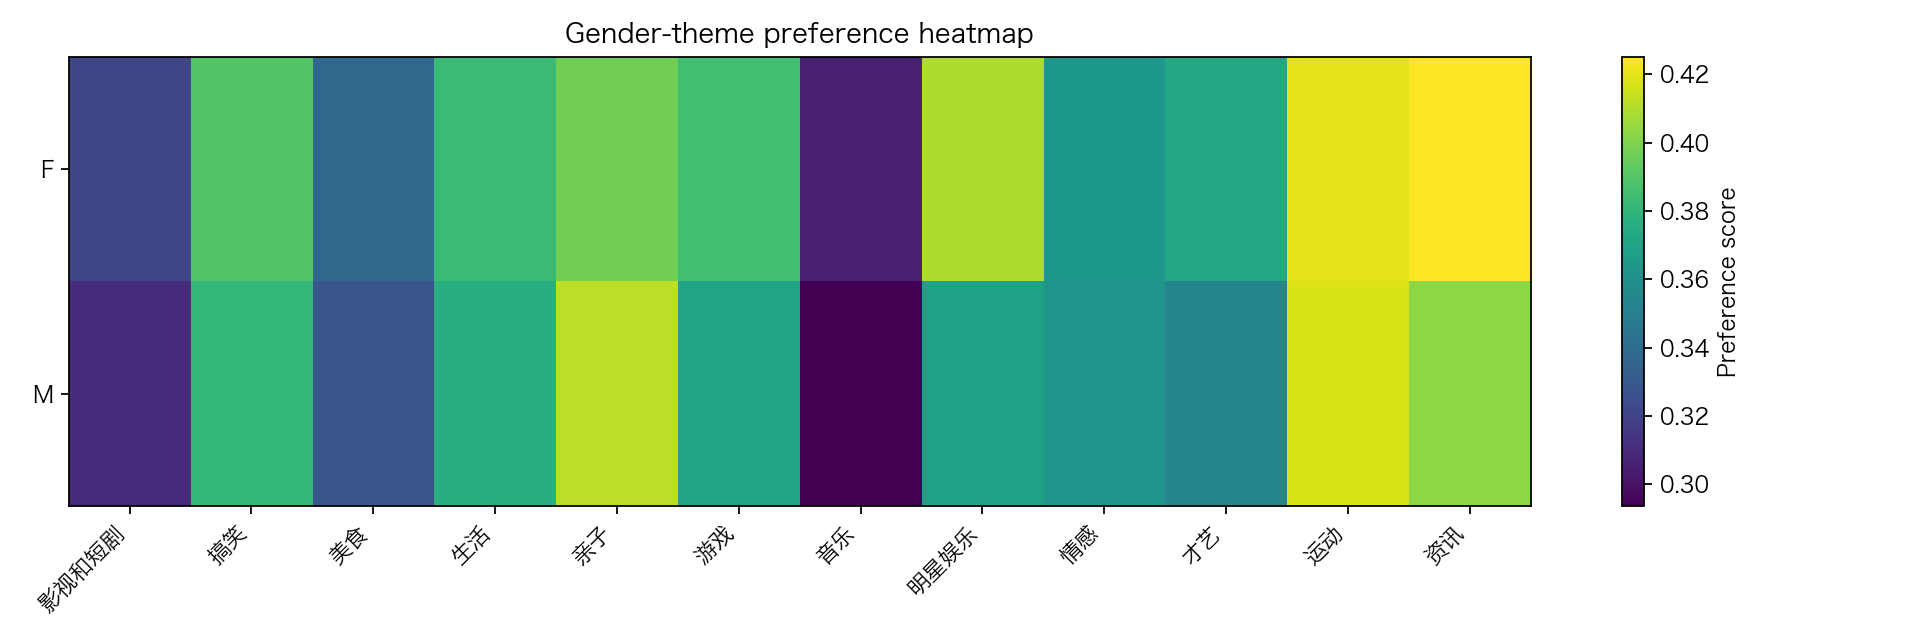
\includegraphics[width=0.86\textwidth]{../../output/figures/gender_theme_preference_heatmap.png}
\caption{性别-主题偏好热力图}
\label{fig:heatmap}
\end{figure}

\section{大数据工具实现与可复现性}

\subsection{Python 本地流水线}

本地实验由 \path{scripts/run_local_pipeline.py} 执行。脚本从原始抽样 CSV 读取数据，完成布尔字段清洗、观看比例计算、年龄和价格分组、主题映射、用户-视频级去重、训练测试切分、主题统计、用户画像、规则挖掘、推荐排序、评估和图表输出。所有关键结果都写入 \path{data_clean/} 与 \path{output/}，便于报告中的数字回到文件中复核。

\path{scripts/check_outputs.py} 用于检查关键产物是否存在并打印摘要。当前校验结果显示，清洗交互数、主题数、规则数、推荐条数和评估指标均与报告一致。这个脚本是项目复现链条中的质量门：如果输出文件缺失或为空，报告结论不能被视为可验证。

\subsection{Spark 与 Hive 实现}

Spark 脚本位于 \path{spark/theme_preference_spark.py}，实现了分布式版本的主题行为统计和 FP-Growth 规则挖掘。脚本使用 Spark SQL 读取 CSV，派生有效观看和观看比例，按用户、视频和曝光时间聚合记录，再输出主题统计表和规则文件。该版本面向更大规模数据，展示了同一分析逻辑迁移到分布式计算环境的方式。

Hive SQL 位于 \path{hive/shortvideo_analysis.sql}，包含原始交互表、类别映射表、清洗视图、主题行为汇总表、用户主题偏好表和用户分组主题统计表。实际部署时需要根据 HDFS 路径调整 \texttt{LOCATION}。Hive 部分的作用是展示离线数仓处理思路，使课程项目不只停留在本地脚本层面。

\subsection{仓库产物}

项目最终产物分为四类。代码产物包括 Python 本地流水线、Spark 脚本和 Hive SQL；数据产物包括清洗后的交互表、用户画像表和视频目录表；结果产物包括主题统计、用户分组统计、用户主题偏好、规则文件、推荐列表和评估表；展示产物包括可视化图表、README、交接文档和最终 PDF 报告。该结构使报告、代码和结果之间保持可追踪关系。

\section{讨论与改进方向}

实验结果表明，主题级规则和群体偏好可以改善推荐排序，但当前方案仍然是一个面向课程项目的可解释基线。其局限主要体现在三个方面。数据方面，抽样时间窗口较短，无法充分观察用户兴趣变化。候选方面，推荐视频来自训练集中出现过的内容，未覆盖新视频冷启动。模型方面，rule-enhanced 的权重由人工设定，虽然便于解释，但没有通过学习排序或交叉验证自动优化。

后续可以沿三条路径改进。数据层面，可以使用更长时间范围和更完整的交互记录，并保留更多内容侧特征。方法层面，可以引入矩阵分解、双塔召回或学习排序模型，将本文构造的主题规则特征作为可解释侧特征。评估层面，可以增加按用户历史长度、主题热度和城市等级划分的分层评估，判断规则增强对冷启动用户和长尾主题是否更有效。

\section{小组分工}

本项目由四名成员共同完成，分工见表~\ref{tab:roles}。成员顺序按课程提交要求排列。

\begin{table}[H]
\centering
\caption{小组成员分工}
\label{tab:roles}
\begin{tabular}{p{2.5cm}p{11cm}}
\toprule
成员 & 主要任务 \\
\midrule
梁珂 & 负责数据清洗、字段标准化、用户-视频级交互表构建、Hive 表结构设计和离线统计 SQL 编写。 \\
方家烨 & 负责项目选题、研究问题定义、数据集阅读、整体技术路线设计，以及开题与最终报告统筹。 \\
李俊婕 & 负责主题偏好分析、用户分群统计、关联规则挖掘、可视化图表整理和实验结果分析。 \\
刘翔 & 负责推荐策略设计、baseline 与 rule-enhanced 对比实验、评估指标计算、Spark 脚本实现和 GitHub 项目整理。 \\
\bottomrule
\end{tabular}
\end{table}

\section{结论}

本文基于 Tsinghua ShortVideo Dataset 的抽样数据，完成了短视频主题偏好分析与推荐策略优化实验。项目将原始多标签曝光记录清洗为 129,483 条用户-视频级交互，构建了用户主题偏好画像，挖掘出 7,658 条主题、标签、用户属性与行为之间的关联规则，并在严格时间切分下比较 baseline 与 rule-enhanced 两种推荐方法。实验结果显示，rule-enhanced 在四项离线指标上均超过 baseline，说明训练集中的主题规律、分群反馈和标签规则能够对个体历史偏好形成补充。

从课程实践角度看，项目覆盖了大数据处理的主要环节：数据读取、字段清洗、结构化聚合、规则挖掘、推荐排序、离线评估、图表展示和报告输出。Python 流水线保证本地复现，Spark 与 Hive 文件展示了面向大规模数据处理的实现思路，最终仓库保留了代码、清洗结果、统计表、规则、推荐列表、图表和报告，能够支撑课程项目提交与后续扩展。

\section*{项目仓库}

\begin{center}
\url{https://github.com/c0ffee-milk/short-video-theme-recommendation}
\end{center}

\end{document}
